\documentclass[a4paper,12pt,twoside]{scrreprt}
% Autor der Vorlage: Klaus Rheinberger, FH Vorarlberg, 2017-02-20

% Pakete:
\usepackage[utf8]{inputenc}
\usepackage[T1]{fontenc} % Silbentrennung bei Sonderzeichen
\usepackage{graphicx} % Bilder einbinden
\usepackage{wrapfig} % Bilder positionieren
\usepackage[ngerman]{babel} % Deutsche Sprachanpassungen
\usepackage{minted} % Code Highlighting/Import
\usepackage{csquotes} % Anführungszeichen und Zitieren
\usepackage[bindingoffset=8mm]{geometry} % Bindeverlust von 8mm einbeziehen
\usepackage{caption} % Abbildungslegenden
\usepackage{xcolor} % Farbige Hervorhebungen
\usepackage{setspace} % Zeilenabstand
\usepackage[style=authoryear,citestyle=authoryear,backend=biber]{biblatex} % Literaturverweise
\usepackage[
    linktocpage=true,
    pdfauthor={Dominic Luidold},
    pdftitle={TODO}
]{hyperref} % Links -> \href{https://www.wikibooks.org}{Wikibooks home}
\usepackage[nohyperlinks]{acronym} % Abkürzungsverzeichnis

% Einstellungen:
\captionsetup{format=hang, justification=raggedright}
\addbibresource{Zotero.bib}
\setcounter{secnumdepth}{4}
\setcounter{tocdepth}{4} % Tiefe der Gliederung im Inhaltsverzeichnis

% Custom Commands
\renewcommand{\listingscaption}{Quellcode}
\renewcommand\listoflistingscaption{Quellcodeverzeichnis}

% Dokumentenbeginn
\begin{document}
\onehalfspacing % Zeilenabstand 1,5

% Titelblatt:
% \newpage\mbox{}\newpage
\cleardoublepage % force output to a right page
\thispagestyle{empty}
\begin{titlepage}
    \begin{flushright}
    
\includegraphics[width=0.4\linewidth]{images/Logo_FHV.jpg}
    \end{flushright}
    \begin{flushleft}
    \section*{TBD}
    \vspace{1cm}

    Bachelorarbeit II\\
    zur Erlangung des akademischen Grades
    \vspace{0.5cm}

    \textbf{Bachelor of Science in Engineering (BSc)}

    \vspace{1cm}
    Fachhochschule Vorarlberg\newline
    Informatik – Software and Information Engineering

    \vspace{0.5cm}

    Betreut von\newline
    Prof. (FH) Dipl. Inform. Thomas Feilhauer

    \vspace{0.5cm}

    Vorgelegt von\newline
    Dominic Luidold\newline
    Dornbirn, \colorbox{yellow}{20. Mai 2021}
    \end{flushleft}
\end{titlepage}

% Widmung:
\newpage
\section*{Widmung}
\label{sec:widmung}
TODO

\bigskip

\begin{quote}
    \begin{flushright}
        \textit{\enquote{TODO}}\\
        TODO
    \end{flushright}
\end{quote}

% Kurzreferat:
\newpage
\section*{Kurzreferat}
\label{sec:kurzreferat}

\subsection*{TODO}

TODO

% Abstract:
\newpage
\section*{Abstract}
\label{sec:abstract}

\subsection*{TODO}

TODO

% Geschlechtergerechte Sprache:
\newpage
\section*{Geschlechtergerechte Sprache}
\label{sec:gendern}

Der Verfasser der vorliegenden Arbeit bekennt sich zu einer geschlechtergerechten Sprachverwendung.

Um die Lesbarkeit zu gewährleisten und zugunsten der Textökonomie werden die verwendeten Personen beziehungsweise Personengruppen fix männlich oder weiblich zugeordnet. Zum Beispiel wird immer \enquote{die Entwicklerin} und \enquote{der Benutzer} verwendet. Es wurde besonders darauf geachtet, stereotype Rollenbeschreibungen zu vermeiden. Die insgesamt eventuell dadurch hervorgerufene Irritation bei den Lesenden ist gewünscht und soll dazu beitragen, eine Bewusstheit für die bestehende, Frauen diskriminierende Sprachgewohnheit (generelle Verwendung der männlichen Begriffe für beide Geschlechter) zu wecken beziehungsweise zu stärken.

% Inhaltsverzeichnis:
\cleardoublepage % force output to a right page
\setcounter{tocdepth}{2}
\tableofcontents

\clearpage
\phantomsection
\addcontentsline{toc}{chapter}{Abbildungsverzeichnis}
\listoffigures

% Abkürzungsverzeichnis:
\clearpage
\phantomsection
\addcontentsline{toc}{chapter}{Abkürzungsverzeichnis}
\chapter*{Abkürzungsverzeichnis}
\begin{acronym}
  \acro{AJAX}{Asynchronous JavaScript and XML}
  \acro{DOM}{Document Object Model}
  \acro{JSON}{JavaScript Object Notation}
  \acro{MPA}{Multi-page Application}
  \acro{PWA}{Progressive Web App}
  \acro{SSR}{Server-side rendering}
  \acro{SPA}{Single-page Application}
  \acro{UI}{User Interface}
  \acro{UX}{User Experience}
\end{acronym}

\chapter{Einleitung}
\label{chap:einleitung}
Diese Bachelorarbeit verfolgt das Ziel, einen Einblick in die \ac{SPA} Frameworks \textit{Angular}\footnote{\href{https://angular.io/}{Angular (https://angular.io)}} und \textit{Vaadin}\footnote{\href{https://vaadin.com/}{Vaadin (https://vaadin.com)}} zu geben und deren Gemeinsamkeiten, Unterschiede sowie Vor- und Nachteile zu beleuchten.

\medskip

Um ein grundlegendes Verständnis über die Thematik von \aclp{SPA} zu erlangen, wird zu Beginn der Arbeit auf das Konzept einer \ac{SPA} eingegangen und die zugrundeliegende Herangehensweise mit der einer klassischen \ac{MPA} verglichen. Im weiteren Verlauf werden die unterschiedlichen Ansätze von Angular und Vaadin genauer betrachtet und eine tatsächliche Umsetzung der zuvor erläuterten Technologien mittels zweier Demo-Applikationen getestet. Am Ende dieser Arbeit wir darauf eingegangen, ob sich - anhand unterschiedlicher Kriterien und Anwendungsfälle - eine Empfehlung für eines der beiden \acs{SPA} Frameworks aussprechen lässt.

\section{Motivation}
\label{sec:motivation}
In den letzten Jahren lässt sich beobachten, dass Webapplikationen, Apps und Anwendungen allgemein verstärkt mittels des \acs{SPA}-Ansatzes umgesetzt werden und somit auf einen Thin Client - im Gegensatz zu klassischeren \aclp{MPA} - setzen. Für die Umsetzung einer solchen Applikation stehen eine Vielzahl von Frameworks zur Verfügung, die darüber hinaus weitere Features bieten und \colorbox{yellow}{Entwickler:innen} bei der Umsetzung unterstützen.

\newpage

Die richtige Wahl des Frameworks, der jeweiligen Technologien und der im Hintergrund agierenden Strukturen spielen eine wesentliche Rolle bei der Planung und Umsetzung eines neuen Projektes. Welches Framework sich besser eignet, lässt sich oftmals nicht auf den ersten (oder sogar zweiten) Blick feststellen. Diese Arbeit befasst sich daher genauer mit dem Konzept von \aclp{SPA} und vergleicht zwei darauf aufbauende Frameworks, die mit deutlich unterschiedlichen Technologie-Stacks arbeiten und zu vergleichbaren Lösungen führen.

\section{Problemstellung}
\label{sec:problemstellung}
Die in Abschnitt \ref{sec:motivation} auf Seite \pageref{sec:motivation} angesprochene Vielzahl an \acs{SPA}-Frameworks bietet grundlegend den Vorteil, dass eine große Auswahlmöglichkeit und eine gewisse Konkurrenz untereinander zu einem hohen Qualitätsstandard führt. Zudem wird dadurch sichergestellt, dass es für jedes Projekt - unabhängig von den jeweiligen Anforderungen und etwaigen Eigenheiten - eine Möglichkeit gibt, dieses mit einem der verfügbaren Frameworks umzusetzen. Auf der anderen Seite führt die stetig wachsende Anzahl an Möglichkeiten jedoch dazu, dass sich meist nur schwer beurteilen lässt, welches Framework sich für die Umsetzung einer Applikation bestmöglich eignet.

\begin{figure}[ht]
    \centering
    
\includegraphics[scale=0.5]{images/js-frameworks.png}
    \caption[Liste möglicher JavaScript-Frameworks zur Umsetzung von \aclp{SPA}]{Liste möglicher JavaScript-Frameworks zur Umsetzung von \aclp{SPA} (Quelle: \cite{a_best_2020})}
    \label{fig:js-frameworks}
\end{figure}

Um eine geeignete Wahl eines Frameworks treffen zu können, sollten vorab Kriterien und Anforderungen definiert werden, die schlussendlich erfüllt werden müssen. Neben grundlegenden Funktionalitäten, die in den meisten Fällen von einer Vielzahl der Frameworks abgedeckt werden können, stellen sich die projektspezifischen Eigenheiten und vor allem die Auswahl der zugrundeliegenden Technologien als eine der wichtigsten Herausforderungen dar. Diese Entscheidung muss gut überlegt und abgewogen werden, da diese im weiteren Verlauf weitreichende Folgen bei der Umsetzung einer (Web-) Applikation zur Folge hat und sich ein Wechsel nach gestarteter Entwicklung nur unter großem Aufwand umsetzen lässt.

Die in Abbildung \ref{fig:js-frameworks} auf Seite \pageref{fig:js-frameworks} dargestellten Frameworks zeigen eine Auswahl an Frameworks auf, die auf \textit{JavaScript} aufbauen beziehungsweise basieren und somit primär auf dem Client - dem Browser - eingesetzt werden können. \aclp{SPA} lassen sich jedoch nicht nur Frontend-seitig entwickeln (bei denen ein Großteil der Logik auf einem externen Server abläuft), sondern können ebenfalls mittels auf \textit{Java} basierenden Frameworks umgesetzt werden. Bei diesen Frameworks - zu denen unter anderem Vaadin gehört - lässt sich sowohl die Logik als auch das \ac{UI}, stellenweise gänzlich, kombinieren.

Da die unterschiedlichen Ansätze, sowohl hinter Vaadin als auch Angular, gewisse Vor- und Nachteile sowie Tücken mit sich bringen, fällt die Wahl auf eines der beiden \acs{SPA}-fähigen Frameworks auf den ersten Blick nicht leicht. Hinzu kommt die Frage, welches der Frameworks weiterführende Funktionalitäten bietet, um mit geringem Aufwand beispielsweise eine \ac{PWA} umzusetzen oder anwendungsspezifische Daten lokal sowie extern persistieren zu können.

\section{Zielsetzung}
\label{sec:zielsetzung}
Die in den Abschnitten \ref{sec:motivation} und \ref{sec:problemstellung} angeführten Punkte haben aufgezeigt, dass die große Anzahl an Frameworks, mit denen \aclp{SPA} umgesetzt werden können, zwar sehr positiv einzuschätzen ist, die damit verbundenen Probleme bei der Auswahl des richtigen Frameworks werden dadurch jedoch verstärkt. Aufgrund der unterschiedlichen zugrundeliegenden Technologien und einhergehenden Herangehensweisen ist eine bedachte Wahl wichtig.

Diese Arbeit verfolgt daher das Ziel, das JavaScript Framework \textit{Angular} dem auf Java basierenden Framework \textit{Vaadin} gegenüberzustellen und zu vergleichen. Das Ziel ist es, mittels Literatur belegter Vergleiche einen Allgemeinen Überblick über \aclp{SPA} zu geben, diese klassischen Ansätzen gegenüberzustellen und zwei Demo-Applikationen zu entwickeln. Diese Webanwendungen werden dann herangezogen, um anhand von vorab definierten Kriterien feststellen zu können, ob und in wie weit Empfehlungen für eines der beiden Frameworks ausgesprochen werden kann.

\medskip

Um den Fokus dieser Arbeit genauer zu definieren und einzuschränken, wird die Planung, Umsetzung sowie abschließenden Beurteilung der Applikationen anhand der ausgearbeiteten Kriterien auf folgende Punkte beschränkt:
\begin{itemize}
    \item Möglichkeit zur einfachen Umsetzung einer \acf{PWA}
    \item Möglichkeit der Wiederverwendbarkeit von Komponenten, gegebenenfalls mittels \textit{Web Components}
    \item Möglichkeit Daten lokal (Browser) sowie extern (Server) zu persistieren
\end{itemize}
\chapter{Stand der Technik}
\label{chap:stand-techni
k}
Das folgende Kapitel gibt einen Überblick über die Funktionsweise einer \acl{SPA} und vergleicht das Konzept von \acsp{SPA} mit klassischen \aclp{MPA}. Im Anschluss wird im Detail auf die Funktionsweise von Angular und Vaadin beziehungsweise deren unterschiedlichen Ansätze in Hinblick auf Entwicklung der \acs{UI} mittels JavaScript und Java eingegangen. Im weiteren Verlauf werden die damit verbundenen Vor- und Nachteile genauer beleuchtet.

\section{Konzept einer \acl{SPA}}
\label{sec:konzept-spa}
Eine klassische \acl{MPA} basiert auf dem Konzept, dass bei jedem Aufruf eines neuen View beziehungsweise einer HTML-Seite eine Anfrage an den Server gestellt wird. Dieser verarbeitet die Anfrage und retourniert das jeweils neu zusammengestellte Resultat der Präsentations- sowie der darunterliegenden Schichten an den Client. Eine \acl{SPA} ist hingegen eine Webanwendung, bei der die Präsentationsschicht und die damit verbundene Logik vom Server entkoppelt und vollständig in den Client, sprich den Browser, ausgelagert wird. \parencite[][Seite 5ff.]{scott_spa_2015}

Die Abbildung \ref{fig:spa-overview} auf Seite \pageref{fig:spa-overview} stellt den Aufbau solch einer \acs{SPA} schematisch dar und verdeutlicht, dass die Darstellung der mittels \acs{AJAX} und XHR angeforderten Daten komplett vom Client übernommen wird. Serverseitig wird lediglich ein \textit{Controller} benötigt, welcher die übermittelten Daten in für die Logik entsprechend verständliche Objekte umwandeln kann.

\medskip

Diese Herangehensweise führt dazu, dass beim Aufrufen einer (Unter-)Seite keine komplett neue HTML-Seite geladen werden muss, sondern lediglich Teile des \acl{UI} - sogennante \textit{Views} - ausgetauscht werden. Hierfür wird das entsprechende \ac{DOM} mittels JavaScript dynamisch ausgetauscht und die benötigten Daten werden bei Bedarf asynchron mittels \acs{AJAX} und XHR vom Server geladen. \parencite[][Seite 7]{scott_spa_2015}

\begin{figure}[ht]
    \centering
    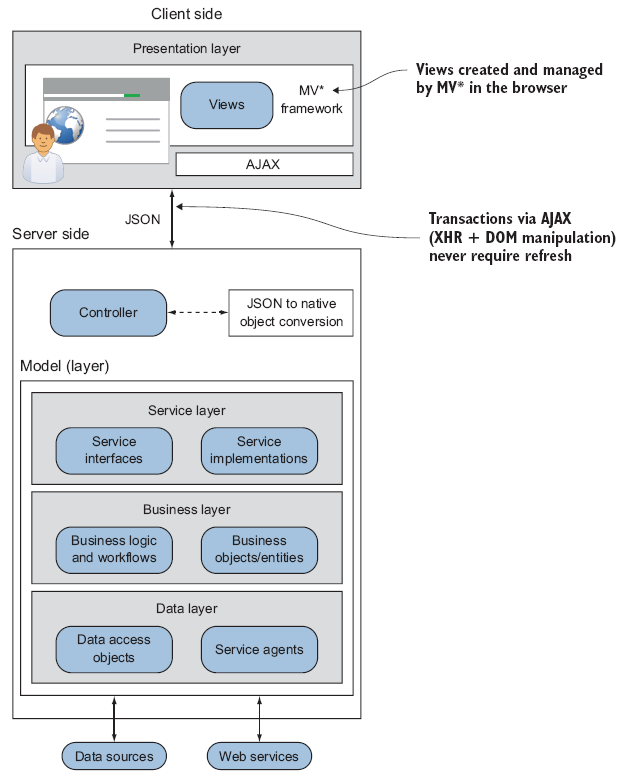
\includegraphics[scale=0.60]{images/SPA_overview_Scott.png}
    \caption[Aufbau einer \acl{SPA}]{Aufbau einer \acl{SPA}\newline(Quelle: \cite[][Seite 6]{scott_spa_2015})}
    \label{fig:spa-overview}
\end{figure}

\subsection{\acl{SSR}}
\label{subsec:ssr}
Neben der reinen Übertragung von Daten mittels \acs{JSON} (oder anderweitigen Datenformaten) kann bei \acsp{SPA} alternativ beziehungsweise erweiternd auch auf \textbf{\ac{SSR}} gesetzt werden. Bei diesem Ansatz werden Ausschnitte von HTML bereits auf dem Server vorbereitet und zusammen mit weiterführenden Daten an den Client geschickt. Dieser kann somit ein Teil der Antwort ohne weitere Aufbereitung darstellen, während die restlichen Daten mittels \acs{DOM}-Manipulation in die View eingebettet werden. \parencite[][Seite 7]{scott_spa_2015}

\subsection{Bestandteile einer \acs{SPA}}
\label{subsec:spa-bestandteile}
Der zugrundeliegende Aufbau einer \acl{SPA} - und der Bestandteil der Applikation, der lediglich einmal geladen wird - ist die sogenannte \textit{Shell}. Die Shell ist eine einzelne HTML-Datei, welche vom Browser vollständig geladen wird und in den meisten Fällen lediglich minimale Strukturen sowie einen leeren \texttt{DIV} Tag enthält, wie Abbildung \ref{fig:spa-shell} auf Seite \pageref{fig:spa-overview} zeigt. Genutzt wird diese als Ausgangspunkt für alle weiteren Views, die unabhängig von der Shell agieren und dynamisch geladen werden. \parencite[][Seite 8]{scott_spa_2015}

\begin{figure}[ht]
    \centering
    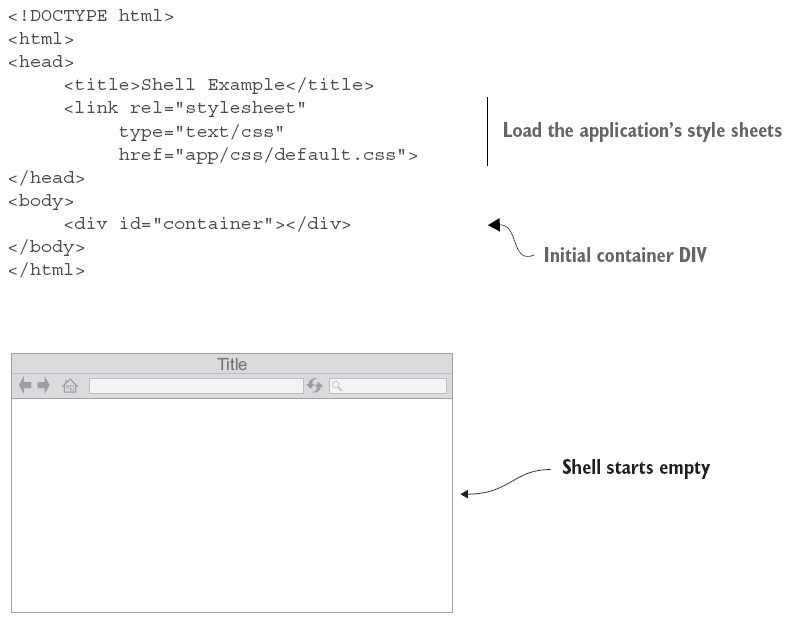
\includegraphics[scale=0.5]{images/SPA_shell_Scott.png}
    \caption[\acl{SPA} Shell]{\acl{SPA} Shell\newline(Quelle: \cite[][Seite 8]{scott_spa_2015})}
    \label{fig:spa-shell}
\end{figure}

Voneinander getrennt sichtbare Bereiche der Anwendung können im weiteren Verlauf ebenfalls mit \texttt{DIV} Tags abgegrenzt werden und sind dem in der Shell definierten \texttt{DIV} Container untergeordnet. Dies ermöglicht eine logische Gruppierung und das gezielte Austauschen bestimmter Bereiche, sogenannter \textit{Regions}. \parencite[][Seite 9]{scott_spa_2015}

\medskip

Die einzeln dargestellten Views, welche dynamisch ausgetauscht werden können, stellen keine vollständigen HTML-Seiten dar, sondern bilden lediglich gezielt definierte Ausschnitte. Diese Ausschnitte werden bei jedem Navigationsvorgang innerhalb der Website durch das entsprechend eingesetzte Framework ausgetauscht und erfordern kein erneutes Laden der Website. \parencite[][Seite 10f.]{scott_spa_2015}

\section{Vorteile einer \acs{SPA} gegenüber einer \acs{MPA}}
\label{sec:vorteile-spa-mpa}
Der Einsatz und die Entwicklung einer \acl{SPA} bietet sowohl Vorteile für Entwickler:innen als auch Anwender:innen gegenüber der Nutzung einer klassischen \acl{MPA}.

\medskip

Der bereits mehrfach angesprochene Vorgang, lediglich bestimmte Teile beziehungsweise Views der Webanwendung auszutauschen, erhöht die Benutzbarkeit sowie die \ac{UX} laut Mikowski und Powell deutlich. Da keine komplett neue (Unter-)Seite geladen werden muss, entfällt das Aufscheinen einer - abhängig von der Internet- und Servergeschwindigkeit - kurz sichtbaren, weißen Übergangsseite während des Ladeprozesses. Dem Benutzer kann stattdessen ein dynamisch dargestellter Fortschrittsbalken dargestellt werden, der sich bei vorhandener Ladezeit laufend aktualisiert. \parencite[][Seite 21]{mikowski_single_2013}

Scott hebt hervor, dass die Aufteilung in entkoppelte Präsentationsschichten auf dem Client sowie dem Server dazu führt, dass diese unabhängig voneinander gewartet und aktualisiert werden können. Während bei klassischen \acsp{MPA} stellenweise HTML, JavaScript ect. mit serverseitigem Code (beispielsweise \textit{PHP}, \textit{JavaServer Pages}, ...) vermischt werden, kann bei \acsp{SPA} zudem eine gewisse Differenzierung und Abtrennung von HTML, CSS und JavaScript im Frontend erzielt werden, was die Wartbarkeit ebenfalls erhöht. \parencite[][Seite 13]{scott_spa_2015}

Sowohl Mikowski und Powell als auch Scott gehen des Weiteren darauf ein, dass die Datenübertragung und Verarbeitung bei einer \acl{SPA} effizienter und schneller stattfinden kann, als bei einer \acl{MPA}. Die Programmlogik zur Darstellung und dynamischen Entscheidungsfindung befindet sich beim Client (weshalb dieser Operationen schnell durchführen kann), während der Server lediglich Validierung, Authentifizierung und Datenspeicherung durchführt. \parencite[][Seite 20]{mikowski_single_2013} Zudem sind Transaktionen zwischen Client und Server nach dem Initialen Aufruf der Applikation schneller, da lediglich Daten in einem vorab definierten Datenformat asynchron übertragen und keine komplletten HTML-Seiten samt JavaScript und CSS ausgetauscht werden müssen. \parencite[][Seite 21]{mikowski_single_2013}

\section{Funktionsweise von Angular und Vaadin im Vergleich}
\label{}

% Literaturverzeichnis:
\clearpage
\phantomsection
\addcontentsline{toc}{chapter}{Literaturverzeichnis}
\printbibliography

\chapter*{Eidesstattliche Erklärung}
\addcontentsline{toc}{chapter}{Eidesstattliche Erklärung}
Ich erkläre hiermit an Eides statt, dass ich die vorliegende Bachelorarbeit I selbstständig und ohne Benutzung anderer als der angegebenen Hilfsmittel angefertigt habe. Die aus fremden Quellen direkt oder indirekt übernommenen Stellen sind als solche kenntlich gemacht. Die Arbeit wurde bisher weder in gleicher noch in ähnlicher Form einer anderen Prüfungsbehörde vorgelegt und auch noch nicht veröffentlicht.

\vspace{5cm}
\noindent
Dornbirn, am \colorbox{yellow}{20. Mai 2021}\hfill Dominic Luidold

\end{document}
